\documentclass[../main.tex]{subfiles}
\begin{document}
\subsection{Simulations}\label{subsec:simulations}

In the following we will consider diffent timescale transformations (although all sigmoids $\sigma(t)\in(-1,+1)$), in particular:
\begin{itemize}
     \item $s = \text{tanh}(t)$;
     \item $s = \frac{t}{1 + |t|}$;
     \item $s = \frac{t}{\sqrt{1 + t^{2}}}$.
\end{itemize}
From \ref{fig:sigmoids} we emphasize that the $3$ time transformations listed above are sorted in descending order from faster ($\text{tanh}(t)$) to slower ($t\big(\sqrt{1+t^{2}}\big)^{-1}$).
We remark that choosing timescale transformations with different growth rates is in some sense equivalent to the tuning of the rate value $\varepsilon$ in the previous case \ref{sec:critical_rate}.

\begin{figure}[H]
    \centering 
    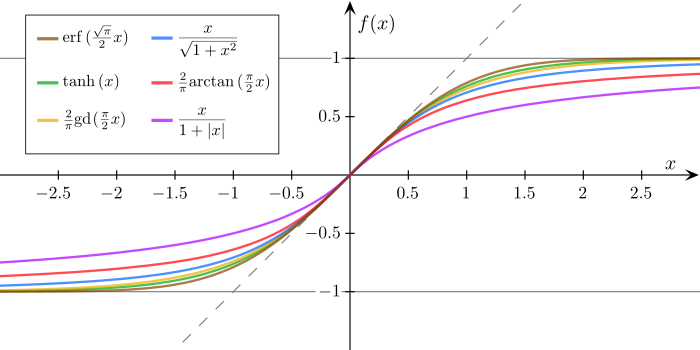
\includegraphics[keepaspectratio, width=\textwidth]{../figures/sigmoids.png}
    \caption{Visualisation of different sigmoid functions $\sigma(t)\in(-1,+1)$. 
    Image taken from \href{https://en.wikipedia.org/wiki/Sigmoid_function\#Examples}{Wikipedia} and to be later replaced by one of your own.}
    \label{fig:sigmoids}
\end{figure}

Finally we hereby provide a closed form expression for the non-autonomous differential equation governing the parameter shift, similar to \eqref{eq:tanh_shift_diff_eq}, for the case of a generic polynomial ramp in the transformed timescale $s = \sigma(t)$

\begin{align}
        g(s) =&\, (g\circ\sigma)(t) = \sum_{k=0}^{n}c_{k}\,\sigma^{k}(t)\nonumber \\
        \dot{\lambda}(t) =&\, \frac{dg}{d\sigma}\frac{d\sigma}{dt} = \sum_{k=1}^{n}c_{k}\,\frac{d}{dt}\sigma^{k}(t) = \Bigg(\sum_{k=1}^{n}k\,c_{k}\,\sigma^{k-1}(t)\Bigg)\dot{\sigma}(t)\, \,. \label{eq:sigm_shift_diff_eq}
\end{align}

% s = tanh(t) 
\subfile{subsubsec:timescale_1}

\end{document}
